\documentclass[twoside,11pt]{article}
\usepackage[utf8]{jmlr2e}

\jmlrheading{Format}{2019}{7}{9/19}{9/19}{Assign1}{Peter Ottsen, Bruce Clark, Justin McGowen, Forest Edwards}

\ShortHeadings{CSCI 447: Machine Learning -- Project 1}{{Ottsen, Clark, McGowen, Edwards}}

\begin{document}

\title{CSCI 447: Machine Learning -- Project 1}

\author{\name Peter Ottsen \email peter.k.ottsen@gmail.com\\
\name Bruce Clark \email brucewestonmt@gmail.com\\
\name Forest Edwards \email forestjedwards@gmail.com\\
\name Justin McGowen \email mcgowen.justin.p@gmail.com}

\editor{None}

\maketitle

\begin{abstract}%

This paper contains the algorithm, experimental approach, results, and discussion of an implementation of a Naive Bayes algorithm \citep{mit15} for predicting classes.  Naive Bayes was the algorithm given for the project due to its relatively straightforward implementation. Five different datasets were used in order to test our model. Once the datasets were cleaned and processed, ten-fold cross-validation was used for each set and the accuracy and precision were recorded. Ten percent of the data in each dataset was then scrambled and ten-fold cross-validation was again used with accuracy and precision being recorded.  The accuracy and precision of the scrambled vs non-scrambled data is discussed and theories for differences are offered.

\end{abstract}

\section{Problem Statement}

Searching for trends and patterns in data can prove to be quite a difficult and time-consuming challenge for data analysts, especially when dealing with very large amounts of data.  An automated method of analysis can be far more beneficial for finding data patterns.  The Naive Bayes algorithm can be very useful tool for this, as it can predict patterns in a dataset with high accuracy.  

In order to get a more accurate prediction for patterns in our data, we hypothesize that running the algorithm on the randomly scrambled data will be less accurate than running it on the unaltered dataset.  We say this because a scrambled sample of data will be less reliable and representative of the features observed.

\section{Description of Algorithm implemented}

The algorithm used in this project was Naive Bayes. Bayes Rule uses probabilities to develop a model for classifying data based on its attributes. It is developed from Bayes Theorem:
\begin{center}
    $P(A|B) = \frac{P(A)*P(B|A)}{P(B)}$
\end{center}
$P(A|B)$ is the probability that A occurs when B occurs. $P(B|A)$ is the probability that B occurs when A occurs. $P(A)$ is the overall probability of A occurring and $P(B)$ is the overall probability of A occurring. \citep{kul11} 

This theorem serves as the basis for the Naive Bayes Algorithm. This algorithm is  "naive" because the assumption is made that the attributes of each class are independent of each other. For example, this means that if a class consists of the attributes X, Y, Z the value of the X attribute has no effect on the value of the Y or Z attribute. This holds for each attribute. \citep{mit15}

The assumption that the position of the arguments does not affect the probability can also be made. Because we are purely looking for the existence or value of an attribute, our data removes position of data already, so this does not have to be taken into account for the equation of the model.

Below is a description of the steps for the training algorithm from the project description given to us.

First we calculate the fraction of the test dataset made up by each of the classes, $c_i$, using the equation below. 
\begin{center}
    $Q(C=c_i) = \frac{#x\epsilon c_i}{N}$
\end{center}
This equation take the number of times class $i$ is seen and divides it by the total number of test data points, $N$.

Each respective class is then taken and the frequency of every attribute value is calculated for that class using the below equation:
\begin{center}
    $F(A_j = a_k, C = c_i) = \frac{#\{x_{A_j} = a_k \wedge (x\ \epsilon \ c_i)\} + 1}{N_{c_i} + d} $
\end{center}
where F is the frequency of attribute $a_k$ for class $c_i$, $#\{x_{A_j} = a_k \wedge (x \epsilon c_i)\}$ is the number of times attribute with value $a_k$ show up in class $c_i$, $N_c_i$ is the number of times class $c_i$ shows up in the training data, and $d$ is the number of attributes. The $1$ is added at the top and $d$ is added on the bottom to smooth the data in case that attribute value does not exist for that class. This is called a Laplace smoother.

From the results of the training algorithm above, the test data is then classified using the below equation:
\begin{center}
    $C(x) = Q(C=C_i) * \prod_{j=1}^d F(A_j = a_k, C = c_i)$
\end{center}
$C(x)$ is a set of values corresponding to the probabilities that the given test data belongs to each class. We then search for the class that has the highest relative probability ie:
\begin{center}
    $class(x) = argmax\ C(x)$
\end{center}
This class, $class(x)$, is then the class our model predicts this test data to be a part of.\citep{she19}

\section{Experimental Approach}

The first thing we did when approaching this project was to examine the data and determined pre-processing was needed. The breast cancer dataset was missing values so we randomly generated attribute values to fill them from the possible values that attribute could hold. The iris and glass datasets contained attribute values that existed in the real number space. These needed to be transformed into discrete values. A Gaussian distribution was used to split the attributes into four equally populated categories for these datasets. If an attribute belonged to the bottom 25\% of values for that attribute, we re-assigned that value as a 1. The top 25\% of values were assigned a 4 and the middle two quartiles were assigned 2 and 3 respectively.

Ten-fold cross-validation was used to test accuracy of the algorithm.  This was useful to do because in examining our individual folds, sometimes the accuracy and precision would be significantly higher or lower than our averages of these two metrics. Each dataset was split into ten sub-sets. Our model made these splits by keeping the same distribution of each class in the sub-sets. By splitting into equally represented class portions, the model minimizes the potential for a class to be unrepresented in the training or test data. Nine of the ten sets were used to train the algorithm and the tenth was used to test the algorithm. This was done ten times over so that each sub-set served as the test data once and training data nine times. 

Data scrambling was used to test the resiliency of the algorithm. Once we tested the algorithm with ten-fold validation for each dataset, ten percent of the original dataset was scrambled to have random attribute values. These scrambled datasets were then tested on the algorithm using the same ten-fold validation method described above.   

The evaluation methods or loss function used were accuracy and precision. These were calculated creating a confusion matrix for each class and using the equations below:
\begin{center}
    $Accuracy = \frac{\#TruePositive + \#TrueNegative}{\# Of TestData}$\\
\end{center}

\begin{center}
    $Precision = \frac{\#TruePositive}{\#TruePositive + \#FalsePositive}$\\
\end{center}

A TruePositive was counted by finding records that belonged to a class that our model predicted it was. 

A TrueNegative was counted by finding records was guessed to not belong to a certain class and the model was correct.

A FalsePositive was counted by finding records that the model guessed to be a certain class but the record did not belong to that class.

A FalseNegative was counted by finding records that the model assumed did not belong to a specified class, but the record did belong to it.

These four values generate our confusion matrix. This was used to evaluate the accuracy and precision for each class. Because each dataset was tested 10 times, our model generated 10 precision and accuracy values for each class in each dataset. These values were averaged and those averages are the ones we are reporting on.

\section{Results}

We set out to try to figure out if introducing noise into a dataset would significantly damage the effectiveness of the Naive Bayes model. We tested our datasets with and without noise over a ten-fold cross-validation and evaluated effectiveness with a confusion matrix. The extensive results of these tests can be found in our $results.txt$ folder in our folder. Here is a summary of the data generated by these tests.

The accuracy calculation was generated by looking at the our confusion matrix to see how many the model identified correctly vs did not identify correctly and then by averaging these results for each fold of the ten-fold cross-validation . For example, upon processing the breast cancer dataset through the model we can figure the following:

\begin{center}
\includegraphics[width=10cm]{accuracyCalc.png}
\end{center}

\noindent
Accuracies were calculated ($accuracy = \frac{(TP+TN)}{ALL}$) across the ten-fold cross-validation for the regular and the scrambled data. Comparing the average of the accuracies for the regular versus scrambled, shows that in general our scrambled data was less accurate than our regular data except in the glass dataset (See table below). The drop in accuracy was expected, so the glass dataset is an outlier. 

\begin{figure}[htp]
    \centering
    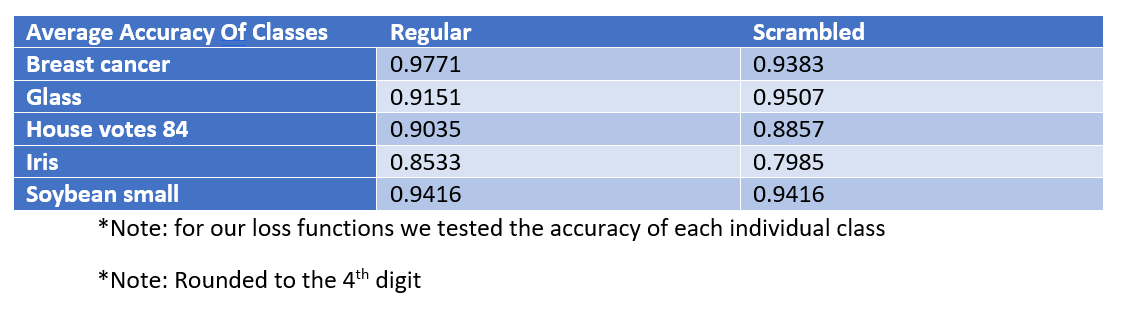
\includegraphics[width=10cm]{table1Accuracy.png}
\end{figure}

Taking a look at these results side by side shows differences in results we get upon scrambling our data. Here we can clearly see the differences between three of the datasets- iris \citep{fis88}, breast cancer \citep{wol87}, soybean \citep{mic87}.


\begin{center}
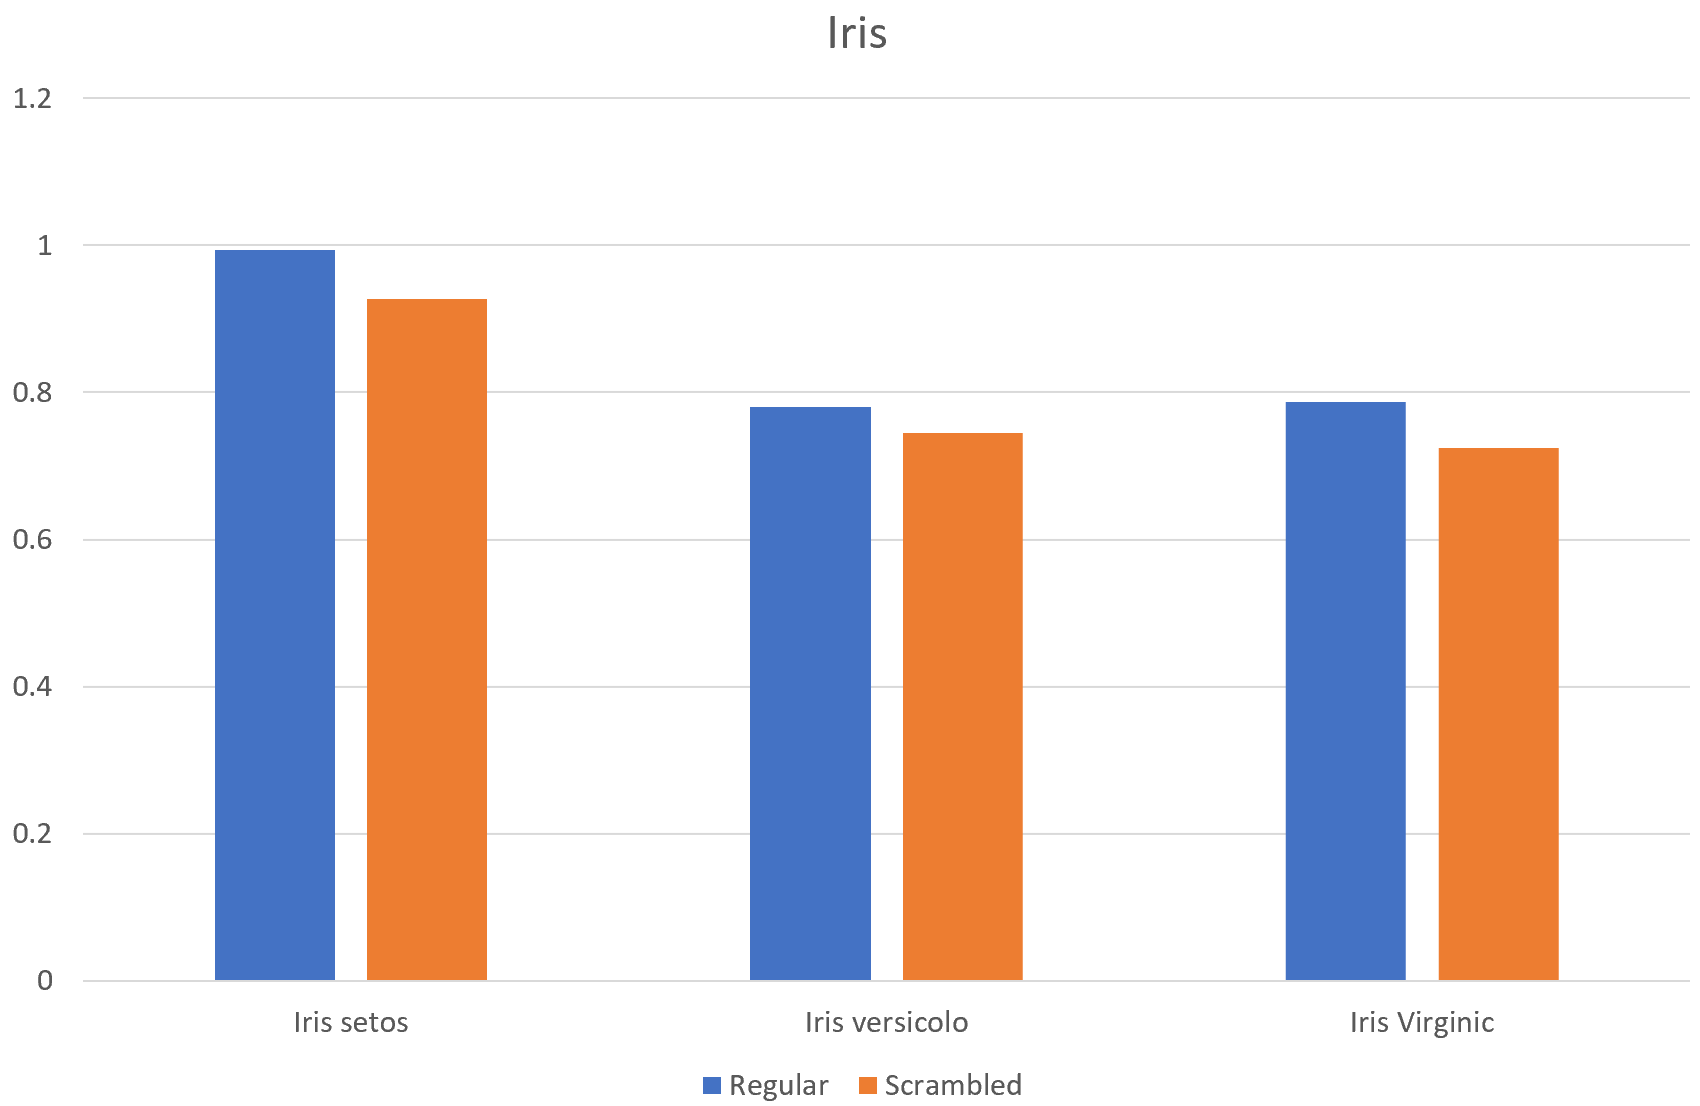
\includegraphics[width=10cm]{iris.png}
\end{center}

\begin{center}
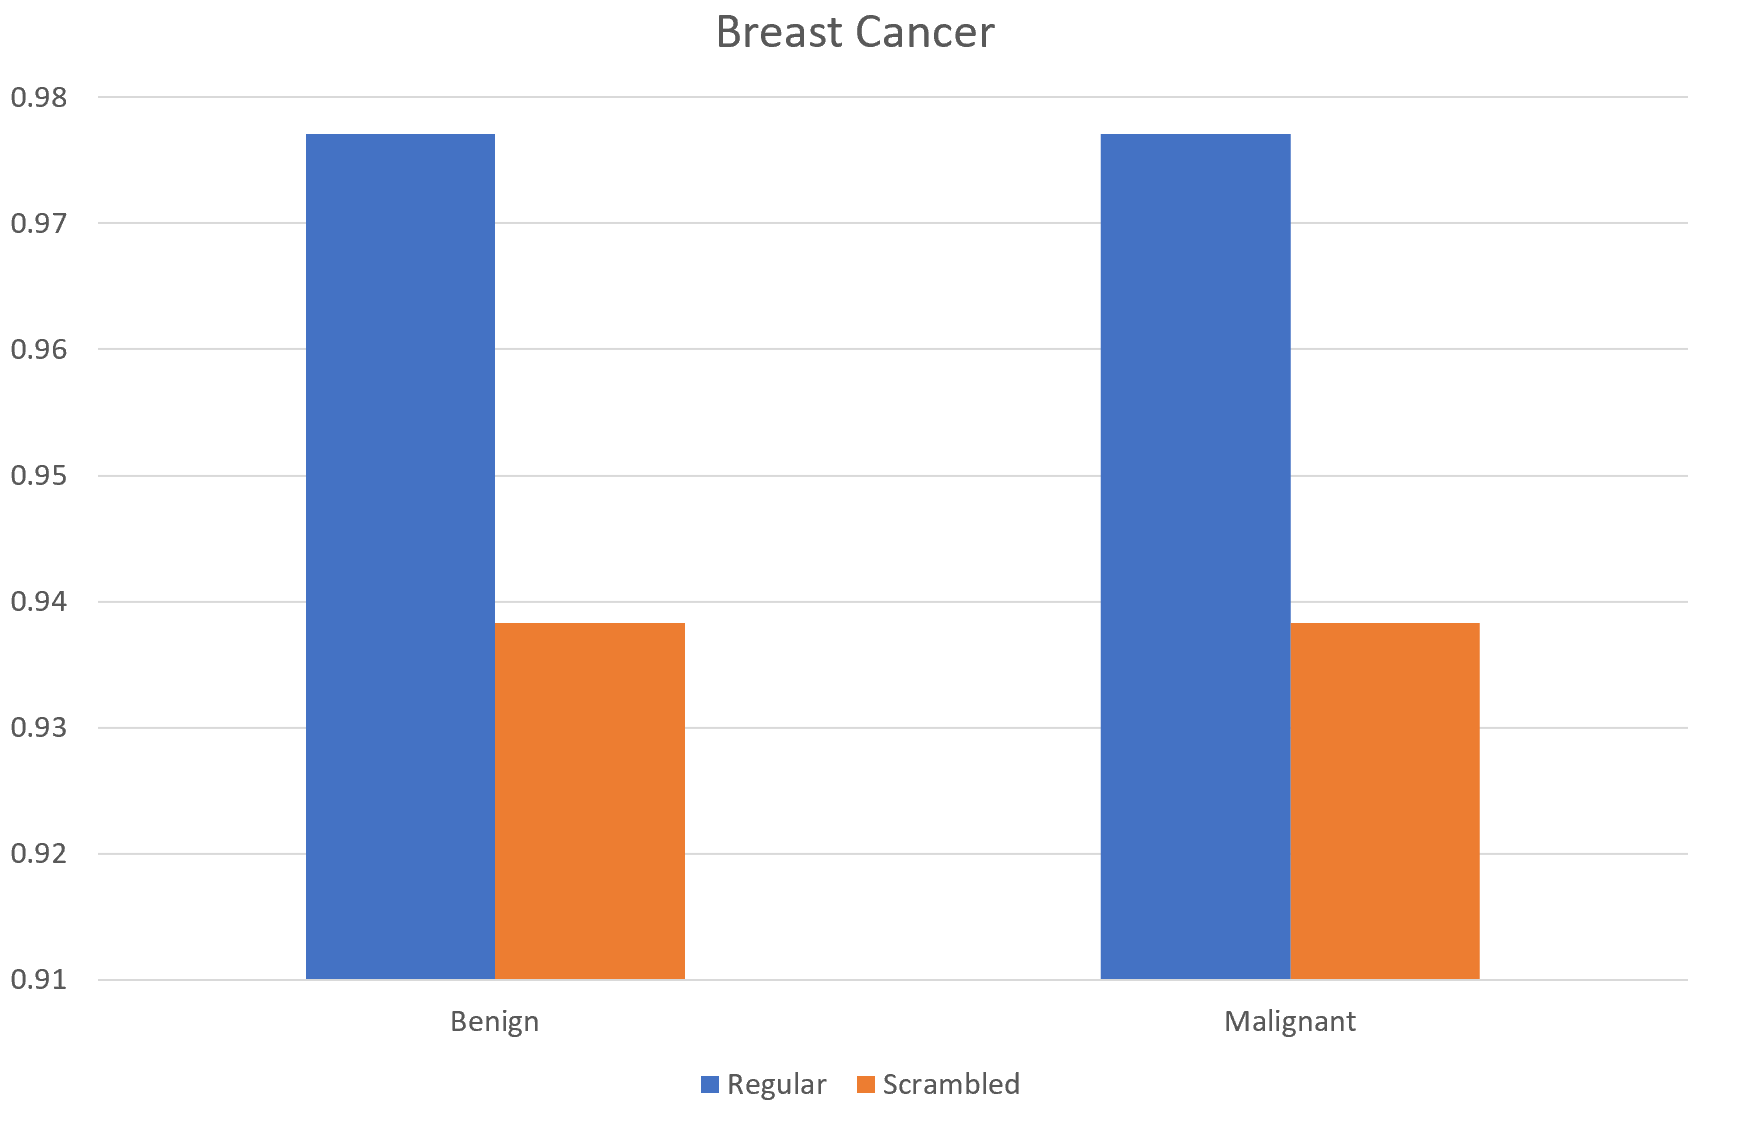
\includegraphics[width=10cm]{breastCan.png}
\end{center}

\begin{center}
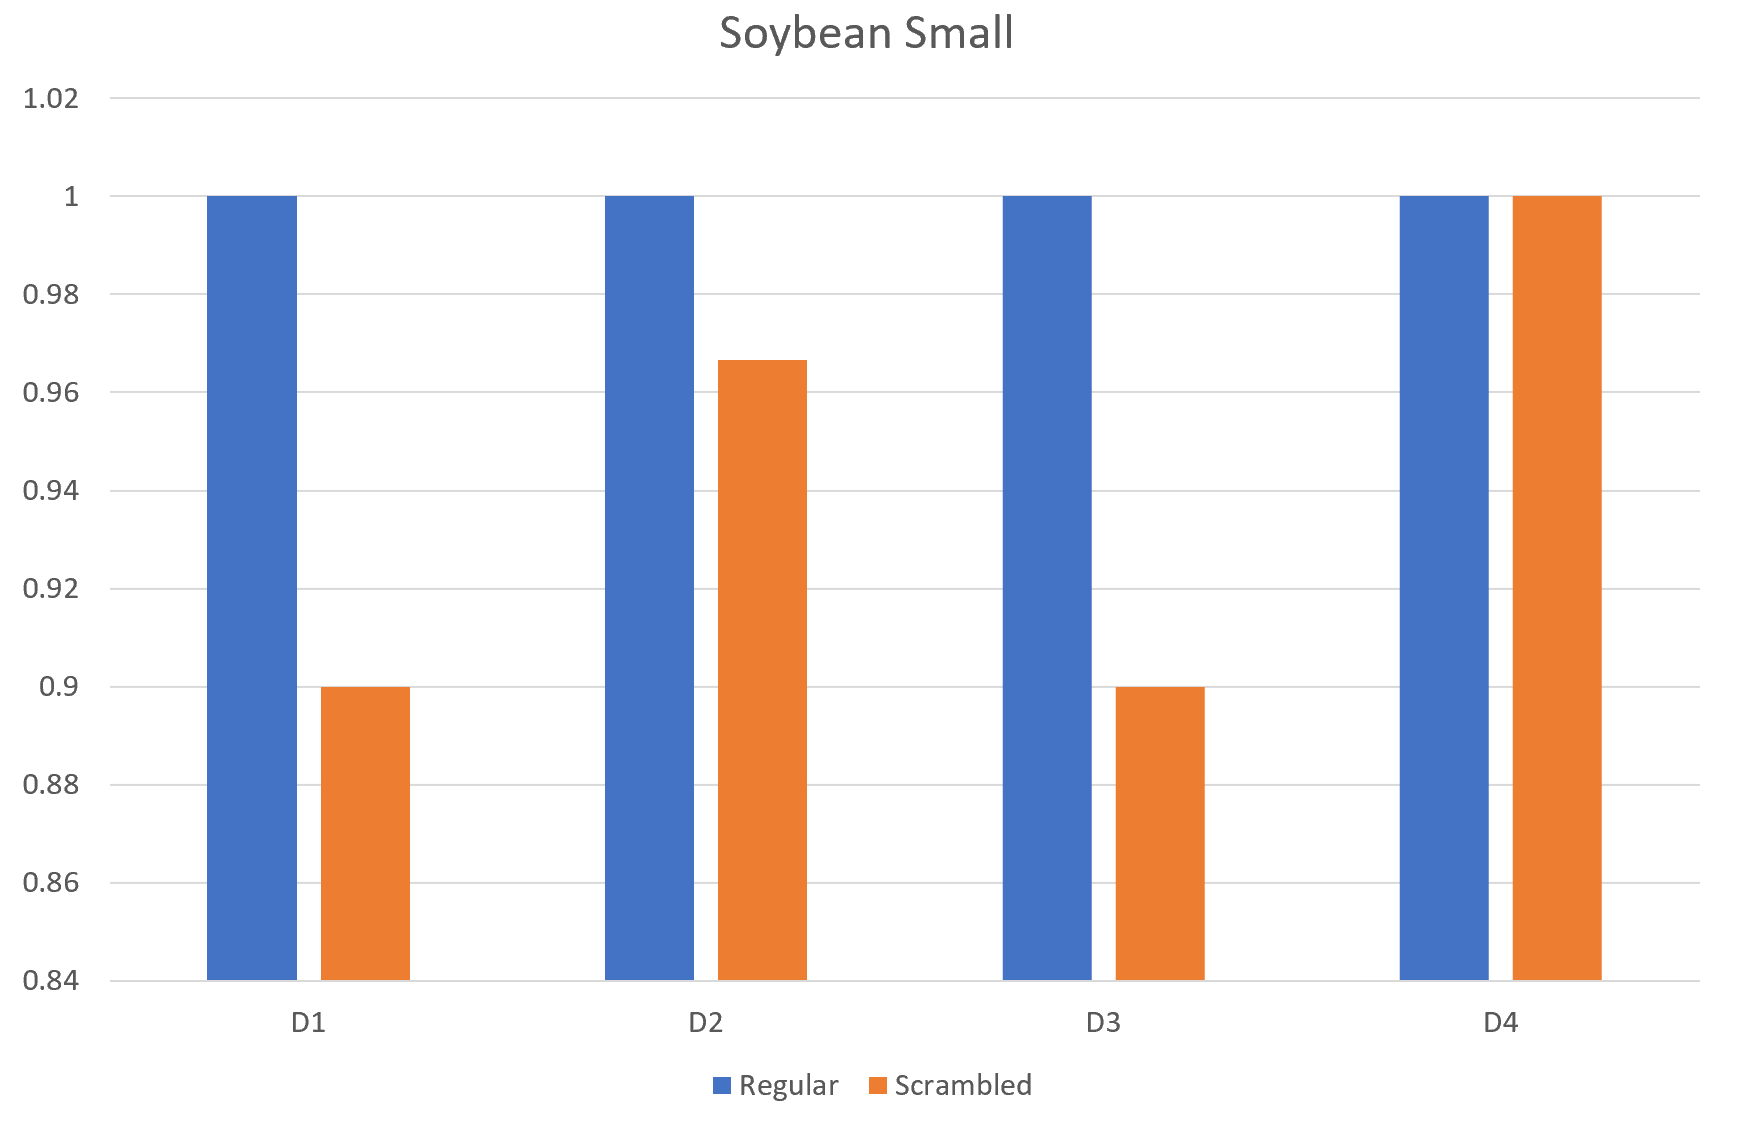
\includegraphics[width=10cm]{soybean.png}
\end{center}





\section{Discussion}

Despite testing over some datasets where classes were not conditionally independent, the prediction model preformed very well at predicting a given class. Even with data that had 10\% random records, the accuracy of these runs never dropped below 70\%. This is an interesting observation because the Naive Bayes model assumes that attributes and classes are conditionally independent.

The algorithm developed usually had a slight decrease in effectively predicting the correct class when we introduced randomized data to our dataset. This was consistent with our hypothesis that the efficiency would decrease when including random data. When we introduced scrambled data, our dataset would contain 10\% randomized data. What is interesting is that most of the time, the accuracy of predicting the classes of datasets with random data was not 10\% less than the accuracy of data that was not randomized. This is shown by the bar graphs in the results section - clean data versus introduction of noise. 

An interesting outlier in the data was the model predicting the class correctly more often in the glass dataset when randomized values were introduced. One potential explanation for this is that the some of the attributes listed in the glass dataset were not strong indicators and did not contribute the predictive model of our algorithm. By randomizing a tenth of our dataset, we introduced noise which allowed for less predictive and applicable attributes to be more flexible and not nullify the ability to predict of our model.\citep{ger87}.

Naive Bayes assumes classes and attributes are independent. We know that two of the three classes in Iris\citep{fis88} are not independent of each other. When predicting these classes, the class that is independent of the other two was predicted with over 90\% accuracy. What is surprising is that the two classes that are not linearly independent of each other were still able to be predicted with over 70\% accuracy. Although this is quite a bit lower, our model still does significantly well for the classes not being independent.

In the soybeans dataset\citep{mic87}, we noticed that some of the classes are strictly dependent on certain attributes. An example of this would be that attribute \#26 is only value 2 when the class is D2. This was the set where our model was able to predict the class 100\% accurately. This leads us to draw the conclusion that this type of classification is more accurate when attributes have a stronger force on determining the class. 

This is also the dataset where noise affected our data the most. We noticed up to a 10\% accuracy difference between our clean data and our data that introduced noise. This may lead to the conclusion that noise in attribute collection where these attributes strongly affect the class of this data is more crucial than when the attributes don't have a strong affect on the class. 

Based on the results discussed above we see that datasets with strong relationships between attributes and classes are influenced by variance in the correctness of our data much more than datasets with weaker relationships. The soybeans set, we were able to predict perfectly when our data was clean and we didn't have noise in our data. However, we noticed some significant drops in efficiency when noise was introduced. In the glass dataset, we actually observe our results improving when noise is implemented to the data. This is possibly due to the fact that randomizing attributes with weaker ties to the class decreases the affect that these attributes have on determining our class, hence improving our results.



\section{Summary}

Overall, we observe Naive Bayes theory to be fairly accurate for predicting classes of data. Even though some of the datasets that the model was tested over did not meet the assumptions for Baye's Rule. Knowing this was a potential issue, we still wanted to see how Naive Bayes would perform.  

The five datasets given needed to be cleaned, so where needed attribute values were added and discretized based on Gaussian distribution in equally populated bins. Ten-fold cross-validation was used to test the algorithm for each of the five datasets. After the cross-validation was run on the datasets, 10\% of each dataset was randomized and the ten-fold cross-validation rerun with the randomized data. As expected this gave a slight decrease in the accuracy of our model except in the glass dataset. This is most likely due to how strong an indicator a given attribute is for predicting the class.

Attributes with stronger ties to determining class seem to be more easily influenced by inaccuracies in data collection. Since data is not perfect in the real world. Measurement errors and missing values introduce noise into our datasets. Because this model is not perfectly resilient to imperfect data, it is important to look at ways we can tune this model and other learning models to improve how well machines can predict information.

\bibliography{references}
\nocite{*}

\end{document}
